%%%%%%%%%%%%%%%%%%%%%%%%%%%%%%%%%%%%%%%%%%  不使用 authblk 包制作标题  %%%%%%%%%%%%%%%%%%%%%%%%%%%%%%%%%%%%%%%%%%%%%%
%-------------------------------PPT Title-------------------------------------
\title{模型微调简介}
%-----------------------------------------------------------------------------

%----------------------------Author & Date------------------------------------
\author[]{\vskip +10pt 姜\;\;骏\inst{}} %[]{} (optional, use only with lots of authors)
%% - Give the names in the same order as the appear in the paper.
%% - Use the \inst{?} command only if the authors have different
%%   affiliation.
\institute[BCC]{\inst{}%
%\institute[Gain~Strong]{\inst{}%
\vskip -15pt 北京市计算中心}
%\vskip -20pt {\large 格致斯创~科技}}
\date[\today] % (optional, should be abbreviation of conference name)
{	{\fontsize{6.2pt}{4.2pt}\selectfont{\textcolor{blue}{E-mail:~}\url{jiangjun@bcc.ac.cn}}}
\vskip 45 pt {\fontsize{8.2pt}{6.2pt}\selectfont{%清华大学\;\;物理系% 报告地点
	\vskip 5 pt \textrm{2025.02}}}
}

%% - Either use conference name or its abbreviation
%% - Not really information to the audience, more for people (including
%%   yourself) who are reading the slides onlin%%   yourself) who are reading the slides onlin%%   yourself) who are reading the slides onlineee
%%%%%%%%%%%%%%%%%%%%%%%%%%%%%%%%%%%%%%%%%%%%%%%%%%%%%%%%%%%%%%%%%%%%%%%%%%%%%%%%%%%%%%%%%%%%%%%%%%%%%%%%%%%%%%%%%%%%%

\subject{}
% This is only inserted into the PDF information catalog. Can be left
% out.
%\maketitle
\frame
{
%	\frametitle{\fontsize{9.5pt}{5.2pt}\selectfont{\textcolor{orange}{“高通量并发式材料计算算法与软件”年度检查}}}
\titlepage
}
%-----------------------------------------------------------------------------

%------------------------------------------------------------------------------列出全文 outline ---------------------------------------------------------------------------------
\section*{}
\frame[allowframebreaks]
{
	\frametitle{\textrm{Outline}}
%  \frametitle{\textcolor{mycolor}{\secname}}
  \tableofcontents%[current,currentsection,currentsubsection]
}
%在每个section之前列出全部Outline
%类似的在每个subsection之前列出全部Outline是\AtBeginSubsection[]
%\AtBeginSection[]
%{
%  \frame<handout:0>%[allowframebreaks]
%  {
%    \frametitle{Outline}
%%全部Outline中,本部分加亮
%    \tableofcontents[current,currentsection]
%  }
%}

%-----------------------------------------------PPT main Body------------------------------------------------------------------------------------
\small
\section{大模型微调}
% 大模型微调的基本概念
\begin{frame}
    \frametitle{通用大模型}
    \textcolor{red}{通用大模型:}~{\fontsize{8.2pt}{6.2pt}\selectfont{如\textrm{GPT}、\textrm{LLaMA}、\textrm{DeepSeek}}}
\begin{figure}[h!]
\vspace*{-0.05in}
\centering
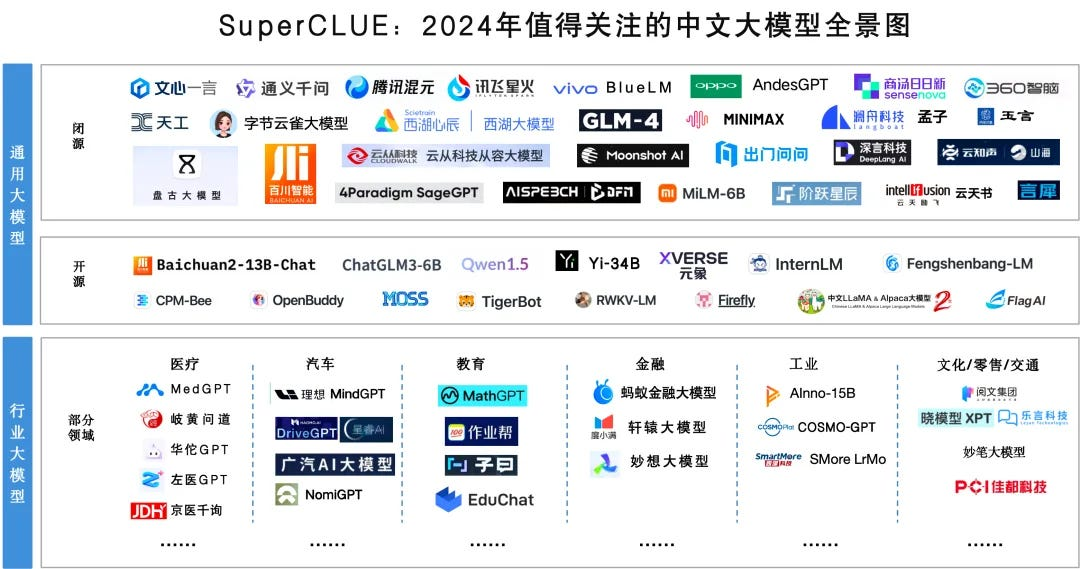
\includegraphics[height=2.0in, width=4.0in, viewport=0 0 1080 510,clip]{Figures/LLM_model-logo_Chinese.jpg}
%\caption{\tiny \textrm{Pseudopotential for metallic sodium, based on the empty core model and screened by the Thomas-Fermi dielectric function.}}%(与文献\cite{EPJB33-47_2003}图1对比)
\label{LLM_model-logo_Chinese}
\end{figure}
\textcolor{blue}{具备强大的通用知识和语言理解能力,预训练参数规模巨大}
\end{frame}

\begin{frame}
    \frametitle{通用模型的局限}
\begin{itemize}
	\item \textcolor{blue}{专业知识深度不足:}\\
		{\fontsize{7.2pt}{6.2pt}\selectfont{通用大模型虽然具有广泛的知识,但对于特定领域的专业知识,知识深度往往不如专门针对该领域训练的模型}}\\
		%{\fontsize{7.2pt}{6.2pt}\selectfont{例如在医学领域,通用大模型可能对一些常见疾病有一定了解,但对于罕见病、复杂的病理机制以及最新的医学研究成果等方面的知识可能不够准确和深入}}
	\item \textcolor{blue}{领域特定语言理解不准确:}\\
		{\fontsize{7.2pt}{6.2pt}\selectfont{不同领域有其独特的术语、概念和语言表达。通用大模型可能难以准确理解和处理这些领域特定语言,导致在文本生成、问答等任务中出现错误或不恰当的回答}}
		%{\fontsize{7.2pt}{6.2pt}\selectfont{以法律领域为例,法律条文和法律文书中的专业术语和特定句式具有严格的法律含义,通用大模型可能无法准确把握这些细节,会影响对法律文本的理解和分析}}
	\item \textcolor{blue}{数据偏差和不完整性:}\\
		{\fontsize{7.2pt}{6.2pt}\selectfont{通用大模型的训练数据来源广泛,但在某些领域可能存在数据偏差或不完整性的问题}}%。如果训练数据中某一领域的样本数量不足或代表性不够,模型在该领域的表现就会受到影响}}
		%{\fontsize{7.2pt}{6.2pt}\selectfont{比如在天文学领域,由于相关数据的获取较为困难,通用大模型在处理天文学特定问题时,可能因数据不足而无法提供准确和全面的解答}}
	\item \textcolor{blue}{缺乏领域特定的逻辑和推理能力:}\\
		{\fontsize{7.2pt}{6.2pt}\selectfont{特定领域往往有其独特的逻辑和推理规则,通用大模型可能无法很好地掌握这些规则}}
		%{\fontsize{7.2pt}{6.2pt}\selectfont{例如在数学领域,进行复杂的数学证明和推理需要遵循严格的数学逻辑,通用大模型可能难以像专业的数学软件或经过专门训练的数学模型那样进行严谨的逻辑推导}}
	\item \textcolor{blue}{无法适应领域的快速变化:}\\
		{\fontsize{7.2pt}{6.2pt}\selectfont{一些特定领域的知识和技术发展迅速,通用大模型可能无法及时跟上这些变化}}
		%{\fontsize{7.2pt}{6.2pt}\selectfont{例如在人工智能领域本身,新的算法、模型和研究成果不断涌现,通用大模型可能无法及时更新其知识体系,从而在处理最新的人工智能相关问题时显得力不从心}}
	\item \textcolor{blue}{计算资源和效率问题:}\\
		{\fontsize{7.2pt}{6.2pt}\selectfont{通用大模型规模一般都较为庞大,在处理特定领域的任务时,可能会存在计算资源消耗过大、运行效率低下的问题}}
		%{\fontsize{7.2pt}{6.2pt}\selectfont{对于一些对实时性要求较高的特定领域应用,如工业自动化控制、金融高频交易等,通用大模型可能无法满足其对响应速度和计算效率的要求}}
\end{itemize}
\end{frame}

\begin{frame}
    \frametitle{通用模型的微调}
    \textcolor{red}{微调:}~在预训练模型基础上,通过\textcolor{magenta}{特定数据集}训练,调整部分或全部参数,以适应特定任务或领域
微调能适配特定任务或领域,{\fontsize{7.2pt}{6.2pt}\selectfont{(如法律文书分析、医疗诊断助手)}} 提升特定场景的应用性能
\begin{figure}[h!]
\vspace*{-0.05in}
\centering
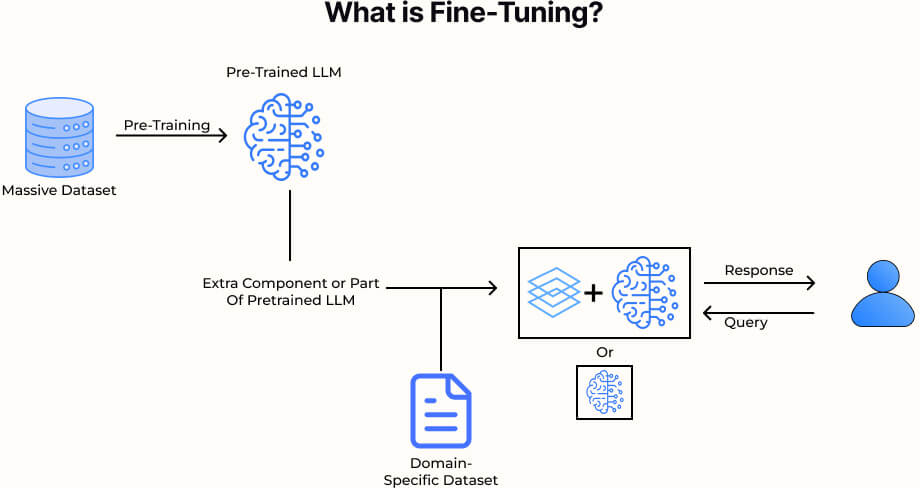
\includegraphics[height=2.1in, width=3.8in, viewport=0 0 220 120,clip]{Figures/What-is-Fine-Tuning.jpg}
%\caption{\tiny \textrm{Pseudopotential for metallic sodium, based on the empty core model and screened by the Thomas-Fermi dielectric function.}}%(与文献\cite{EPJB33-47_2003}图1对比)
\label{What-is-Fine-Tuning}
\end{figure}
\vskip -0.15in
\end{frame}

\begin{frame}
    \frametitle{通用模型的微调}
\begin{figure}[h!]
\vspace*{-0.10in}
\centering
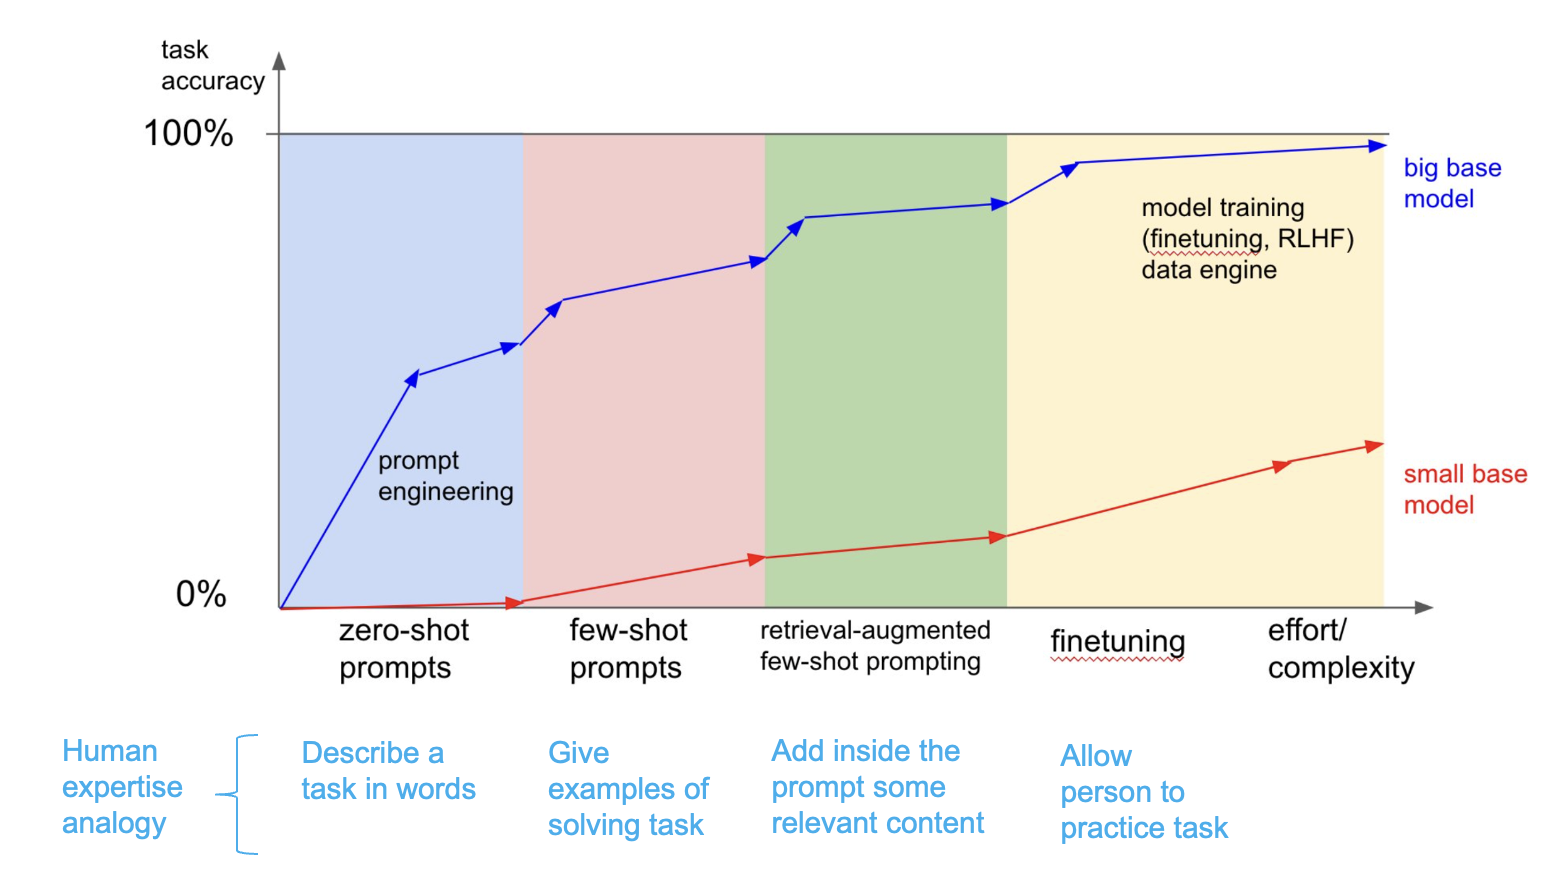
\includegraphics[height=2.1in, width=3.7in, viewport=0 0 790 460,clip]{Figures/Human_expertise_analogy.png}
%\caption{\tiny \textrm{Pseudopotential for metallic sodium, based on the empty core model and screened by the Thomas-Fermi dielectric function.}}%(与文献\cite{EPJB33-47_2003}图1对比)
\label{Human_expertise_analogy}
\end{figure}
\vskip -0.05in
微调能适配特定任务或领域,{\fontsize{7.2pt}{6.2pt}\selectfont{(如法律文书分析、医疗诊断助手)}} 提升特定场景的应用性能
\end{frame}

\section{方法、工具与流程}
\subsection{大模型微调的方法}
% 大模型微调的方法
\begin{frame}
    \frametitle{大模型微调的方法}
    \begin{itemize}
	    \item \textcolor{purple}{基于特征提取的微调:}\\
		    {\fontsize{7.2pt}{6.2pt}\selectfont{冻结预训练模型大部分层,仅训练新添加分类器或回归层,适用于数据量小、任务与预训练任务相关性高的场景,如图像分类任务}}
	    \item \textcolor{purple}{部分层微调:}\\
		    {\fontsize{7.2pt}{6.2pt}\selectfont{选择预训练模型部分层进行微调,平衡训练成本和模型性能,如文本摘要任务}}
	    \item \textcolor{purple}{全模型微调:}\\
		    {\fontsize{7.2pt}{6.2pt}\selectfont{对预训练模型所有参数进行微调,适用于数据量充足、任务与预训练任务差异大的场景,如情感分析任务}}
    \end{itemize}
\begin{figure}[h!]
\vspace*{-0.10in}
\centering
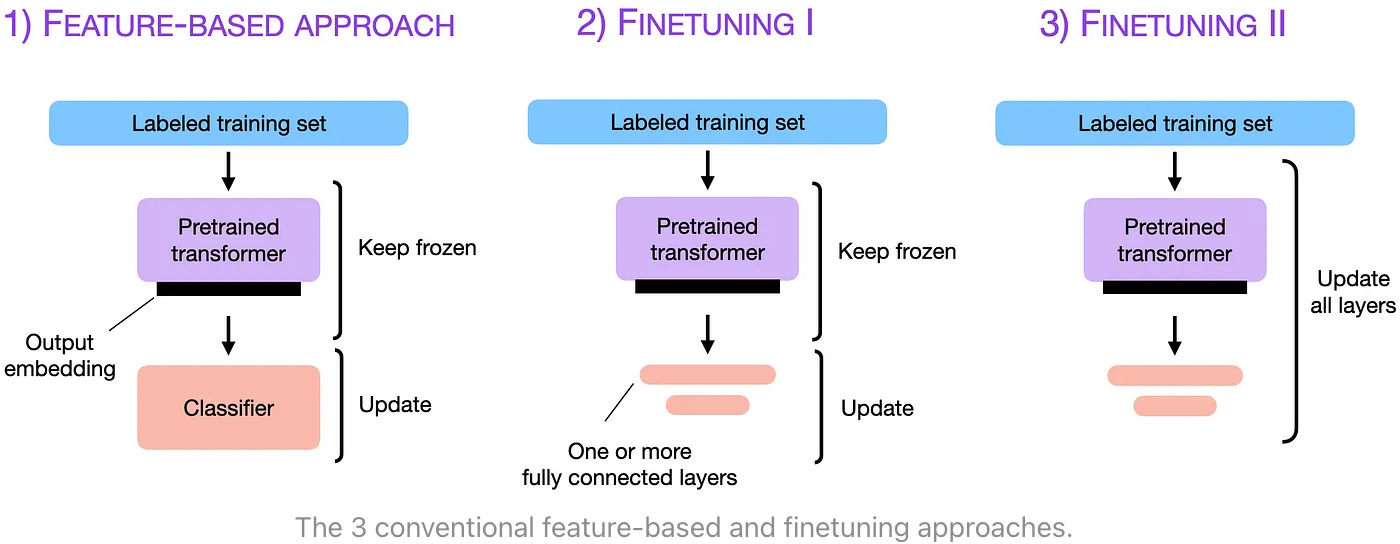
\includegraphics[height=1.3in, width=3.7in, viewport=0 40 1400 544,clip]{Figures/Three_conventional_approaches_fine-tuning_LLM.jpeg}
%\caption{\tiny \textrm{Pseudopotential for metallic sodium, based on the empty core model and screened by the Thomas-Fermi dielectric function.}}%(与文献\cite{EPJB33-47_2003}图1对比)
\label{LLM_model-fine_tuning}
\end{figure}
\end{frame}

\begin{frame}
    \frametitle{参数高效微调}
	    \textcolor{purple}{参数高效微调:}\\
		    {\fontsize{7.2pt}{6.2pt}\selectfont{保持预训练模型大部分参数不变的情况下,通过仅调整少量额外参数来适应新任务的技术}}
\begin{figure}[h!]
\vspace*{-0.05in}
\centering
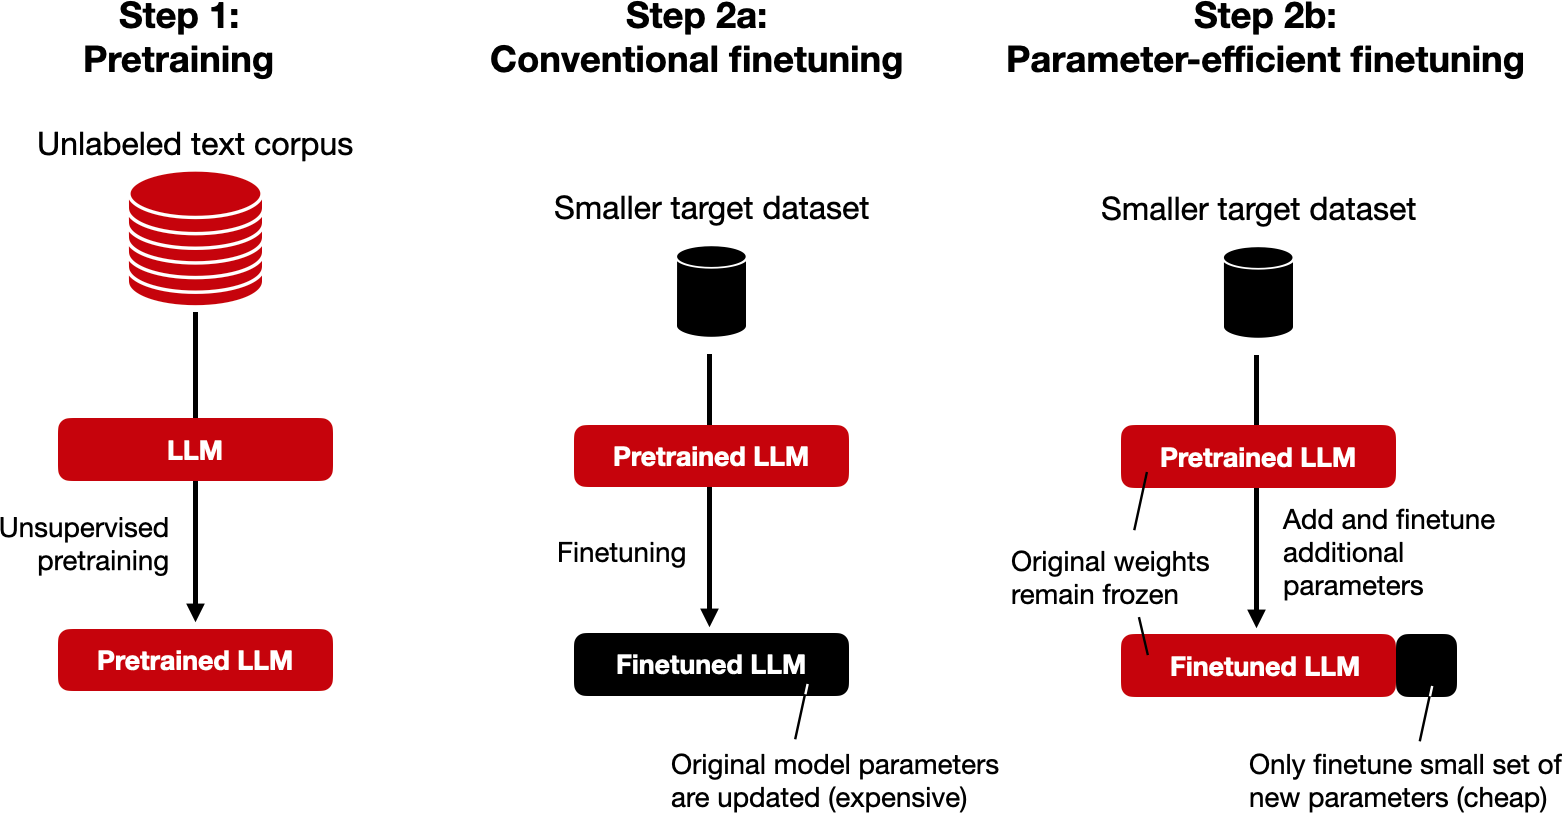
\includegraphics[height=1.8in, width=3.7in, viewport=0 0 1562 778,clip]{Figures/The_idea_of_parameter-efficient_finetuning_techniques.png}
%\caption{\tiny \textrm{Pseudopotential for metallic sodium, based on the empty core model and screened by the Thomas-Fermi dielectric function.}}%(与文献\cite{EPJB33-47_2003}图1对比)
\label{parameter-efficient_finetuning}
\end{figure}
\vskip -0.05in
\textcolor{blue}{这种方法显著降低了计算和内存需求,同时保持了与全参数微调相当的性能}
\end{frame}

\begin{frame}
    \frametitle{参数高效微调}
    \begin{itemize}
	    \item \textcolor{red}{蒸馏\textrm{(distillation):}}\\
		    {\fontsize{7.2pt}{6.2pt}\selectfont{该方法涉及训练一个较小的模型来模仿一个较大的预训练模型的行为}}%。预训练模型生成“教师”预测结果,然后用于训练较小的“学生”模型。通过这样做,学生模型可以从较大模型的知识中学习,而无需存储所有参数。%它由Hinton等人于2015年引入。
	    \item  \textcolor{red}{适配器训练\textrm{(adapter training):}}\\
		    {\fontsize{7.2pt}{6.2pt}\selectfont{适配器是添加到预训练模型中的小型神经网络,用于特定任务的微调}}%。这些适配器只占原始模型大小的一小部分,这使得训练更快,内存需求更低。适配器可以针对多种任务进行训练,然后插入到预训练模型中以执行新任务。%它由Houlsby等人于2019年引入。
	    \item \textcolor{red}{渐进收缩\textrm{(progressive shrinking):}}\\
		    {\fontsize{7.2pt}{6.2pt}\selectfont{这种技术涉及在\textrm{fine-tuning}期间逐渐减小预训练模型的大小}}%。从一个大模型开始,逐渐减少参数的数量,直到达到所需的性能。这种方法可以产生比从头开始训练的模型性能更好的小型模型。%它由Kaplan等人于2020年引入。
    \end{itemize}
\begin{figure}[h!]
\vspace*{-0.08in}
\centering
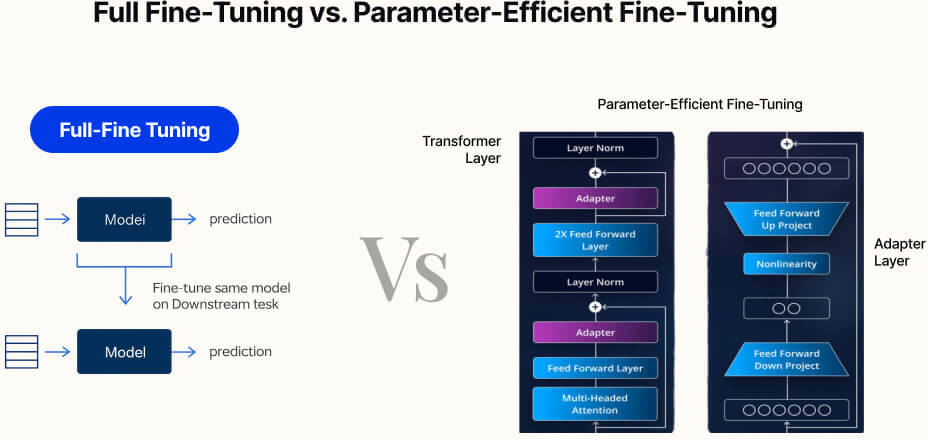
\includegraphics[height=1.6in, width=4.0in, viewport=0 0 225 90,clip]{Figures/Full-Fine-Tuning-vs-Parameter-Efficient-Fine-Tuning.jpg}
%\caption{\tiny \textrm{Pseudopotential for metallic sodium, based on the empty core model and screened by the Thomas-Fermi dielectric function.}}%(与文献\cite{EPJB33-47_2003}图1对比)
\label{Full-Fine-Tuning-vs-Parameter-Efficient-Fine-Tuning}
\end{figure}
\end{frame}

\begin{frame}
    \frametitle{提示语微调}
	    \textcolor{purple}{提示语微调:~}{\fontsize{7.2pt}{6.2pt}\selectfont{重点是调整输入提示\textrm{(input prompt)}而非修改模型参数
	    \begin{itemize}
		    \item 预训练模型保持不变,只有输入提示被修改以适应下游的任务
		    \item 通过设计和优化一组提示,可以使预训练模型执行特定任务
	    \end{itemize}
	    \textrm{prompt-tuning}调整比精调的计算成本低,需要的资源和训练时间也更少
    }}
\begin{figure}[h!]
\vspace*{-0.05in}
\centering
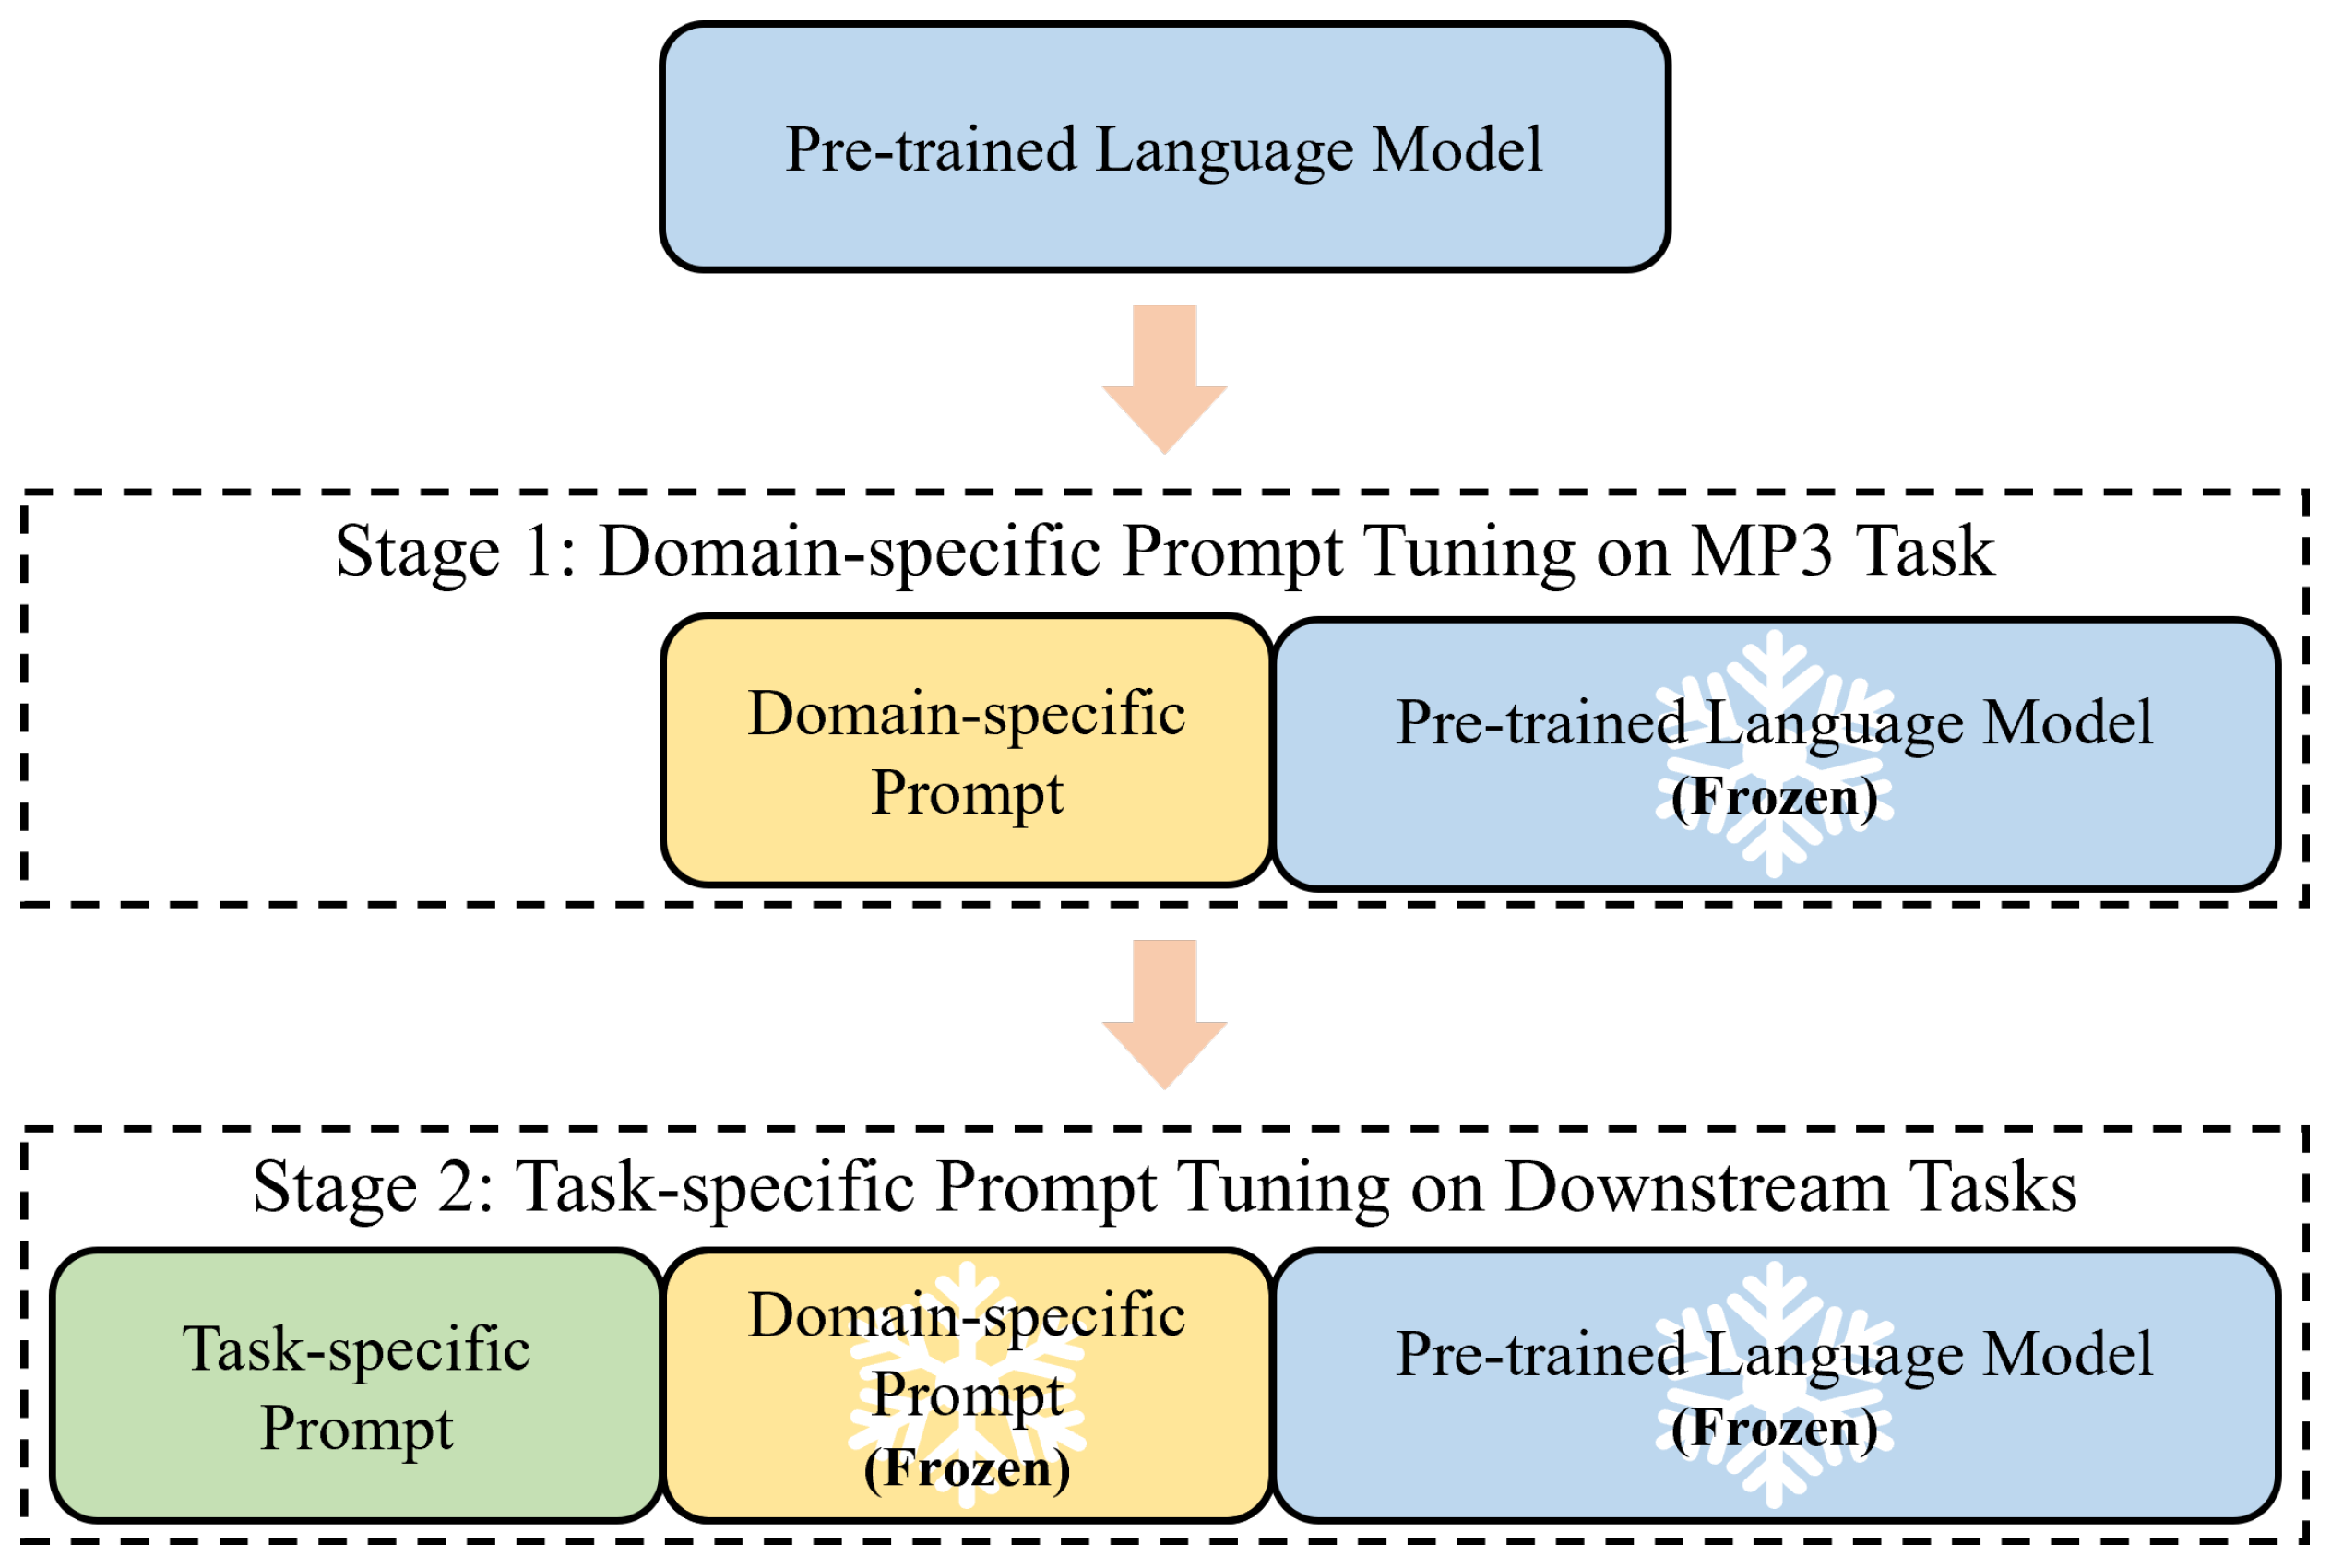
\includegraphics[height=1.4in, width=2.3in, viewport=0 0 327 205,clip]{Figures/Multi-stage_prompt_tuning_strategy.png}
%\caption{\tiny \textrm{Pseudopotential for metallic sodium, based on the empty core model and screened by the Thomas-Fermi dielectric function.}}%(与文献\cite{EPJB33-47_2003}图1对比)
\label{Multi-stage_prompt_tuning_strategy}
\end{figure}
\vskip -0.05in
\textcolor{blue}{\textrm{prompt-tuning}和传统的\textrm{fine-tuning}的主要区别:}\\
{\fontsize{7.2pt}{6.2pt}\selectfont{预训练模型被修改的程度——\\
	~\textrm{fine-tuning}修改模型的权重,\textrm{prompt-tuning}只修改模型的输入}}
\end{frame}


\subsection{大模型微调的工具}
% 大模型微调的工具
\begin{frame}[fragile]
	\frametitle{大模型微调的工具:~\textrm{Hugging Face Transformer}}
	\textcolor{magenta}{\textrm{Hugging Face Transformers}}:\\
	提供丰富预训练模型、简单易用的\textrm{API},支持多种深度学习框架
\begin{figure}[h!]
\vspace*{-0.01in}
\centering
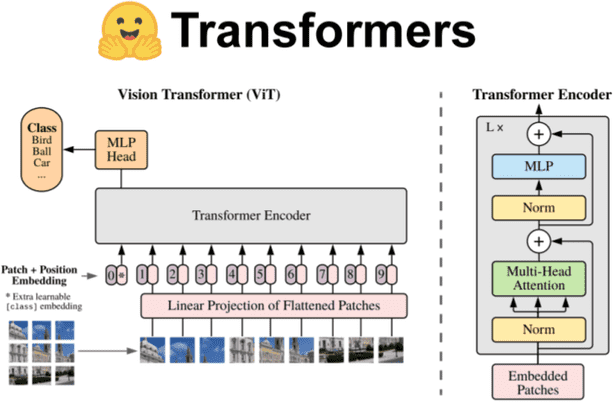
\includegraphics[height=1.1in, width=1.6in, viewport=0 0 613 402,clip]{Figures/hugging-face-vit.png}
%\caption{\tiny \textrm{Pseudopotential for metallic sodium, based on the empty core model and screened by the Thomas-Fermi dielectric function.}}%(与文献\cite{EPJB33-47_2003}图1对比)
\label{hugging-face-vit}
\end{figure}
            \begin{lstlisting}[style=pythonstyle]
# Hugging Face微调示例代码
from transformers import AutoModelForSequenceClassification
from transformers import TrainingArguments, Trainer
model = AutoModelForSequenceClassification.from_pretrained("bert-base-uncased", num_labels = 2)
# 后续训练代码
            \end{lstlisting}
\end{frame}

%\begin{frame}[fragile,allowframebreaks]
%	\frametitle{大模型微调的工具:~\textrm{Hugging Face Transformer}}
%            \begin{lstlisting}[style=pythonstyle]
%import torch
%from torch.utils.data import Dataset, DataLoader
%from transformers import DistilBertTokenizer, DistilBertForSequenceClassification, AdamW
%from sklearn.model_selection import train_test_split
%from tqdm import tqdm
%
%# 自定义数据集类
%class TextClassificationDataset(Dataset):
%    def __init__(self, texts, labels, tokenizer, max_length):
%        self.texts = texts
%        self.labels = labels
%        self.tokenizer = tokenizer
%        self.max_length = max_length
%
%    def __len__(self):
%        return len(self.texts)
%
%    def __getitem__(self, idx):
%        text = str(self.texts[idx])
%        label = self.labels[idx]
%        encoding = self.tokenizer.encode_plus(
%            text,
%            add_special_tokens=True,
%            max_length=self.max_length,
%            padding='max_length',
%            truncation=True,
%            return_tensors='pt'
%        )
%        return {
%            'input_ids': encoding['input_ids'].flatten(),
%            'attention_mask': encoding['attention_mask'].flatten(),
%            'labels': torch.tensor(label, dtype=torch.long)
%        }
%
%# 示例数据
%texts = ["This is a positive sentence.", "This is a negative sentence.", "Another positive one.", "Another negative one."]
%labels = [1, 0, 1, 0]
%
%# 划分训练集和验证集
%train_texts, val_texts, train_labels, val_labels = train_test_split(texts, labels, test_size=0.2, random_state=42)
%
%# 初始化分词器和模型
%tokenizer = DistilBertTokenizer.from_pretrained('distilbert-base-uncased')
%model = DistilBertForSequenceClassification.from_pretrained('distilbert-base-uncased', num_labels=2)
%
%# 创建数据集和数据加载器
%max_length = 128
%train_dataset = TextClassificationDataset(train_texts, train_labels, tokenizer, max_length)
%val_dataset = TextClassificationDataset(val_texts, val_labels, tokenizer, max_length)
%
%train_dataloader = DataLoader(train_dataset, batch_size=2, shuffle=True)
%val_dataloader = DataLoader(val_dataset, batch_size=2, shuffle=False)
%
%# 定义优化器
%optimizer = AdamW(model.parameters(), lr=2e-5)
%
%# 训练模型
%device = torch.device('cuda' if torch.cuda.is_available() else 'cpu')
%model.to(device)
%
%epochs = 3
%for epoch in range(epochs):
%    model.train()
%    total_train_loss = 0
%    for batch in tqdm(train_dataloader):
%        input_ids = batch['input_ids'].to(device)
%        attention_mask = batch['attention_mask'].to(device)
%        labels = batch['labels'].to(device)
%
%        model.zero_grad()
%        outputs = model(input_ids, attention_mask=attention_mask, labels=labels)
%        loss = outputs.loss
%        total_train_loss += loss.item()
%
%        loss.backward()
%        optimizer.step()
%
%    avg_train_loss = total_train_loss / len(train_dataloader)
%    print(f'Epoch {epoch + 1}: Average training loss = {avg_train_loss}')
%
%    # 验证模型
%    model.eval()
%    total_val_loss = 0
%    total_val_accuracy = 0
%    for batch in val_dataloader:
%        input_ids = batch['input_ids'].to(device)
%        attention_mask = batch['attention_mask'].to(device)
%        labels = batch['labels'].to(device)
%
%        with torch.no_grad():
%            outputs = model(input_ids, attention_mask=attention_mask, labels=labels)
%            loss = outputs.loss
%            total_val_loss += loss.item()
%            logits = outputs.logits
%            predictions = torch.argmax(logits, dim=1)
%            total_val_accuracy += (predictions == labels).sum().item()
%
%    avg_val_loss = total_val_loss / len(val_dataloader)
%    avg_val_accuracy = total_val_accuracy / len(val_dataset)
%    print(f'Epoch {epoch + 1}: Average validation loss = {avg_val_loss}, Average validation accuracy = {avg_val_accuracy}')
%
%# 保存微调后的模型
%model.save_pretrained('fine_tuned_model')
%tokenizer.save_pretrained('fine_tuned_model')
%            \end{lstlisting}
%\end{frame}
%    
\begin{frame}[fragile,allowframebreaks]
	\frametitle{大模型微调的工具:~\textrm{TensorFlow Extended}}
%        \column{0.33\textwidth}
%            \centerline{\includegraphics[width=0.8\textwidth]{TFX图标}}
	\textcolor{magenta}{\textrm{TensorFlow Extended~(TFX):}}\\支持端到端模型开发和部署,提供数据预处理、模型训练、评估和部署等功能
%            \includegraphics[width=0.8\textwidth]{TFX微调工作流程图}
\begin{figure}[h!]
\vspace*{-0.10in}
\centering
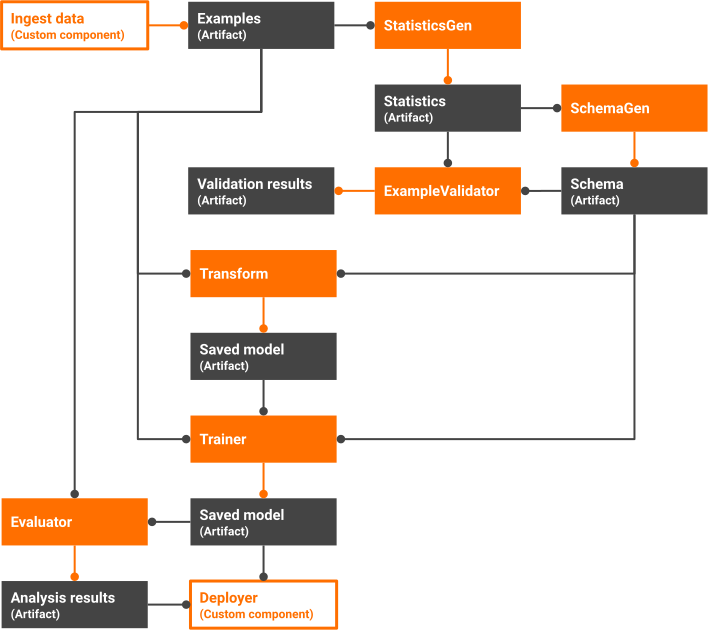
\includegraphics[height=2.2in, width=3.1in, viewport=0 0 600 530,clip]{Figures/TXF_Pipeline.png}
%\caption{\tiny \textrm{Pseudopotential for metallic sodium, based on the empty core model and screened by the Thomas-Fermi dielectric function.}}%(与文献\cite{EPJB33-47_2003}图1对比)
\label{TXF_Pipeline}
\end{figure}
\end{frame}

%\begin{frame}[fragile,allowframebreaks]
%	\frametitle{大模型微调的工具:~\textrm{TensorFlow Extended}}
%            \begin{lstlisting}[style=pythonstyle]
%import os
%import tempfile
%import urllib
%
%import absl
%import tensorflow as tf
%import tensorflow_model_analysis as tfma
%from tfx import v1 as tfx
%from tfx.components import CsvExampleGen
%from tfx.components import Evaluator
%from tfx.components import ExampleValidator
%from tfx.components import Pusher
%from tfx.components import ResolverNode
%from tfx.components import SchemaGen
%from tfx.components import StatisticsGen
%from tfx.components import Trainer
%from tfx.components import Transform
%from tfx.dsl.experimental import latest_blessed_model_resolver
%from tfx.orchestration import metadata
%from tfx.orchestration import pipeline
%from tfx.orchestration.experimental.interactive.interactive_context import InteractiveContext
%from tfx.proto import pusher_pb2
%from tfx.proto import trainer_pb2
%from tfx.types import Channel
%from tfx.types.standard_artifacts import Model
%from tfx.types.standard_artifacts import ModelBlessing
%from typing import Dict, List, Text
%
%# 定义管道参数
%_pipeline_name = 'image_classification_finetuning'
%# 数据路径
%_data_root = tempfile.mkdtemp(prefix='tfx-data')
%_data_url = 'https://raw.githubusercontent.com/tensorflow/tfx/master/tfx/examples/penguin/data/labelled/penguins_processed.csv'
%urllib.request.urlretrieve(_data_url, os.path.join(_data_root, 'data.csv'))
%# 管道根目录
%_pipeline_root = os.path.join(tempfile.mkdtemp(prefix='tfx-pipelines'), _pipeline_name)
%# 模型服务路径
%_serving_model_dir = os.path.join(tempfile.mkdtemp(prefix='tfx-serving'), _pipeline_name)
%# 元数据路径
%_metadata_path = os.path.join(tempfile.mkdtemp(prefix='tfx-metadata'), 'metadata.db')
%
%# 创建交互式上下文
%context = InteractiveContext(pipeline_root=_pipeline_root)
%
%# 1. 数据生成
%example_gen = CsvExampleGen(input_base=_data_root)
%context.run(example_gen)
%
%# 2. 数据统计
%statistics_gen = StatisticsGen(examples=example_gen.outputs['examples'])
%context.run(statistics_gen)
%
%# 3. 数据模式生成
%schema_gen = SchemaGen(
%    statistics=statistics_gen.outputs['statistics'],
%    infer_feature_shape=False)
%context.run(schema_gen)
%
%# 4. 数据验证
%example_validator = ExampleValidator(
%    statistics=statistics_gen.outputs['statistics'],
%    schema=schema_gen.outputs['schema'])
%context.run(example_validator)
%
%# 5. 数据转换
%_transform_module_file = 'penguin_transform.py'
%%%writefile {_transform_module_file}
%
%import tensorflow as tf
%
%_FEATURE_KEYS = [
%    'culmen_length_mm', 'culmen_depth_mm', 'flipper_length_mm', 'body_mass_g'
%]
%_LABEL_KEY = 'species'
%
%def _transformed_name(key):
%    return key + '_xf'
%
%def preprocessing_fn(inputs):
%    """tf.transform's callback function for preprocessing inputs.
%    Args:
%      inputs: map from feature keys to raw not-yet-transformed features.
%    Returns:
%      Map from string feature key to transformed feature operations.
%    """
%    outputs = {}
%
%    # 对特征进行标准化
%    for key in _FEATURE_KEYS:
%        outputs[_transformed_name(key)] = tf.cast(inputs[key], tf.float32)
%    outputs[_transformed_name(_LABEL_KEY)] = tf.cast(inputs[_LABEL_KEY], tf.int64)
%
%    return outputs
%
%transform = Transform(
%    examples=example_gen.outputs['examples'],
%    schema=schema_gen.outputs['schema'],
%    module_file=os.path.abspath(_transform_module_file))
%context.run(transform)
%
%# 6. 模型训练
%_trainer_module_file = 'penguin_trainer.py'
%%%writefile {_trainer_module_file}
%
%import tensorflow as tf
%import tensorflow_transform as tft
%
%from tfx.components.trainer.fn_args_utils import FnArgs
%
%_FEATURE_KEYS = [
%    'culmen_length_mm', 'culmen_depth_mm', 'flipper_length_mm', 'body_mass_g'
%]
%_LABEL_KEY = 'species'
%
%def _transformed_name(key):
%    return key + '_xf'
%
%def _gzip_reader_fn(filenames):
%    """小批量读取压缩文件的函数"""
%    return tf.data.TFRecordDataset(
%        filenames, compression_type='GZIP')
%
%def _input_fn(file_pattern: List[Text],
%              data_accessor: tfx.components.DataAccessor,
%              tf_transform_output: tft.TFTransformOutput,
%              batch_size: int = 200) -> tf.data.Dataset:
%    """生成输入数据集的函数"""
%    dataset = data_accessor.tf_dataset_factory(
%        file_pattern,
%        _gzip_reader_fn,
%        record_format='tfrecord',
%        shuffle=True).repeat()
%
%    transformed_feature_spec = (
%        tf_transform_output.transformed_feature_spec().copy())
%
%    dataset = dataset.map(
%        lambda x: (
%            tf.io.parse_single_example(x, transformed_feature_spec),
%            x[_transformed_name(_LABEL_KEY)]
%        ),
%        num_parallel_calls=tf.data.AUTOTUNE)
%
%    dataset = dataset.batch(batch_size)
%    return dataset
%
%def _build_keras_model() -> tf.keras.Model:
%    """构建一个简单的 Keras 模型用于微调"""
%    inputs = [
%        tf.keras.layers.Input(shape=(1,), name=_transformed_name(f))
%        for f in _FEATURE_KEYS
%    ]
%    d = tf.keras.layers.concatenate(inputs)
%    for _ in range(2):
%        d = tf.keras.layers.Dense(8, activation='relu')(d)
%    outputs = tf.keras.layers.Dense(3, activation='softmax')(d)
%
%    model = tf.keras.Model(inputs=inputs, outputs=outputs)
%    model.compile(
%        optimizer=tf.keras.optimizers.Adam(learning_rate=0.001),
%        loss='sparse_categorical_crossentropy',
%        metrics=[tf.keras.metrics.SparseCategoricalAccuracy()])
%
%    return model
%
%def run_fn(fn_args: FnArgs):
%    """Train the model based on given args.
%    Args:
%      fn_args: Holds args used to train the model as name/value pairs.
%    """
%    tf_transform_output = tft.TFTransformOutput(fn_args.transform_output)
%
%    train_dataset = _input_fn(
%        fn_args.train_files,
%        fn_args.data_accessor,
%        tf_transform_output,
%        batch_size=40)
%    eval_dataset = _input_fn(
%        fn_args.eval_files,
%        fn_args.data_accessor,
%        tf_transform_output,
%        batch_size=40)
%
%    model = _build_keras_model()
%
%    # 加载预训练模型(这里只是示例,实际需要替换为真正的预训练模型)
%    # pretrained_model = tf.keras.models.load_model('pretrained_model_path')
%    # 可以在这里对模型进行微调,例如冻结部分层等操作
%
%    model.fit(
%        train_dataset,
%        steps_per_epoch=fn_args.train_steps,
%        validation_data=eval_dataset,
%        validation_steps=fn_args.eval_steps)
%
%    model.save(fn_args.serving_model_dir, save_format='tf')
%
%trainer = Trainer(
%    module_file=os.path.abspath(_trainer_module_file),
%    examples=transform.outputs['transformed_examples'],
%    transform_graph=transform.outputs['transform_graph'],
%    schema=schema_gen.outputs['schema'],
%    train_args=trainer_pb2.TrainArgs(num_steps=100),
%    eval_args=trainer_pb2.EvalArgs(num_steps=50))
%context.run(trainer)
%
%# 7. 模型评估
%eval_config = tfma.EvalConfig(
%    model_specs=[tfma.ModelSpec(label_key='species_xf')],
%    metrics_specs=[
%        tfma.MetricsSpec(
%            metrics=[
%                tfma.MetricConfig(class_name='SparseCategoricalAccuracy'),
%                tfma.MetricConfig(class_name='AUC')
%            ]
%        )
%    ],
%    slicing_specs=[tfma.SlicingSpec()])
%
%# 找到最新的经过验证的模型
%model_resolver = ResolverNode(
%    instance_name='latest_blessed_model_resolver',
%    resolver_class=latest_blessed_model_resolver.LatestBlessedModelResolver,
%    model=Channel(type=Model),
%    model_blessing=Channel(type=ModelBlessing))
%context.run(model_resolver)
%
%evaluator = Evaluator(
%    examples=example_gen.outputs['examples'],
%    model=trainer.outputs['model'],
%    baseline_model=model_resolver.outputs['model'],
%    eval_config=eval_config)
%context.run(evaluator)
%
%# 8. 模型推送
%pusher = Pusher(
%    model=trainer.outputs['model'],
%    model_blessing=evaluator.outputs['blessing'],
%    push_destination=pusher_pb2.PushDestination(
%        filesystem=pusher_pb2.PushDestination.Filesystem(
%            base_directory=_serving_model_dir)))
%context.run(pusher)
%            \end{lstlisting}
%\end{frame}

\begin{frame}[fragile,allowframebreaks]
    \frametitle{大模型微调的工具:~\textrm{PyTorch Lightning}}
%        \column{0.33\textwidth}
%            \centerline{\includegraphics[width=0.8\textwidth]{PyTorchLightning图标}}
    \textcolor{magenta}{\textrm{PyTorch Lightning}}:\\
    简化\textrm{PyTorch}模型训练过程,提高代码可维护性和可扩展性
\begin{figure}[h!]
\vspace*{-0.05in}
\centering
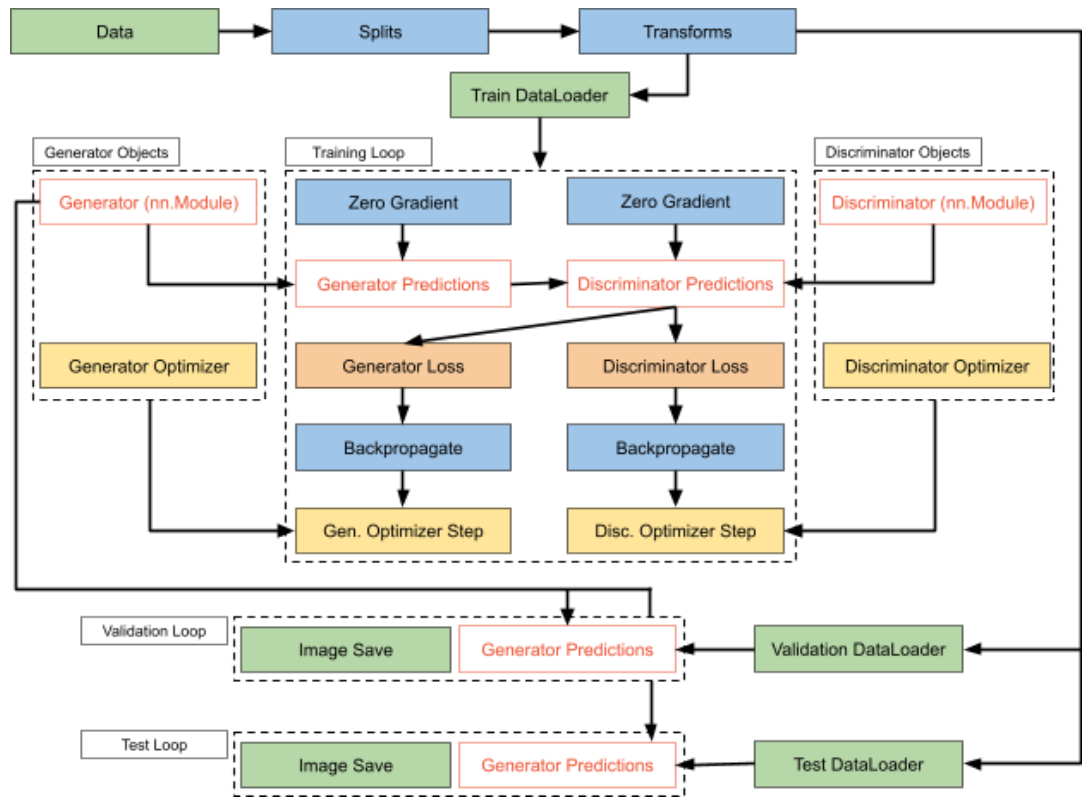
\includegraphics[height=2.2in, width=3.5in, viewport=0 0 590 404,clip]{Figures/Pytorch_Lightning_GAN.png}
%\caption{\tiny \textrm{Pseudopotential for metallic sodium, based on the empty core model and screened by the Thomas-Fermi dielectric function.}}%(与文献\cite{EPJB33-47_2003}图1对比)
\label{Pytorch_Lightning_GAN}
\end{figure}
            \begin{lstlisting}[style=pythonstyle]
# PyTorch Lightning微调示例代码
from pytorch_lightning import LightningModule

class MyModel(LightningModule):

     def __init__(self):
         super().__init__()
  # 模型定义
    def training_step(self, batch, batch_idx):
  # 训练步骤
  # 后续训练代码
            \end{lstlisting}
%    \end{columns}
%    \begin{center}
%        \begin{tabular}{|c|c|c|}
%            \hline
%            工具 & 特点 & 适用场景 \\
%            \hline
%            Hugging Face Transformers & 丰富模型、易用API & 快速原型开发 \\
%            \hline
%            TensorFlow Extended (TFX) & 端到端开发 & 大规模生产场景 \\
%            \hline
%            PyTorch Lightning & 简化训练 & PyTorch开发者 \\
%            \hline
%        \end{tabular}
%    \end{center}
\end{frame}

%\begin{frame}[fragile,allowframebreaks]
%    \frametitle{大模型微调的工具:~\textrm{PyTorch Lightning}}
%            \begin{lstlisting}[style=pythonstyle]
%	    import os
%import torch
%from torch.utils.data import Dataset, DataLoader
%from transformers import BertTokenizer, BertForSequenceClassification
%import pytorch_lightning as pl
%from sklearn.model_selection import train_test_split
%import pandas as pd
%
%
%# 自定义数据集类
%class IMDBDataset(Dataset):
%    def __init__(self, texts, labels, tokenizer, max_length):
%        self.texts = texts
%        self.labels = labels
%        self.tokenizer = tokenizer
%        self.max_length = max_length
%
%    def __len__(self):
%        return len(self.texts)
%
%    def __getitem__(self, idx):
%        text = str(self.texts[idx])
%        label = self.labels[idx]
%        encoding = self.tokenizer.encode_plus(
%            text,
%            add_special_tokens=True,
%            max_length=self.max_length,
%            padding='max_length',
%            truncation=True,
%            return_tensors='pt'
%        )
%        return {
%            'input_ids': encoding['input_ids'].flatten(),
%            'attention_mask': encoding['attention_mask'].flatten(),
%            'labels': torch.tensor(label, dtype=torch.long)
%        }
%
%
%# PyTorch Lightning 模型类
%class SentimentClassifier(pl.LightningModule):
%    def __init__(self, model_name='bert-base-uncased', num_classes=2, lr=2e-5):
%        super(SentimentClassifier, self).__init__()
%        self.model = BertForSequenceClassification.from_pretrained(model_name, num_labels=num_classes)
%        self.lr = lr
%
%    def forward(self, input_ids, attention_mask):
%        outputs = self.model(input_ids=input_ids, attention_mask=attention_mask)
%        return outputs.logits
%
%    def training_step(self, batch, batch_idx):
%        input_ids = batch['input_ids']
%        attention_mask = batch['attention_mask']
%        labels = batch['labels']
%        logits = self(input_ids, attention_mask)
%        loss = torch.nn.functional.cross_entropy(logits, labels)
%        self.log('train_loss', loss)
%        return loss
%
%    def validation_step(self, batch, batch_idx):
%        input_ids = batch['input_ids']
%        attention_mask = batch['attention_mask']
%        labels = batch['labels']
%        logits = self(input_ids, attention_mask)
%        loss = torch.nn.functional.cross_entropy(logits, labels)
%        preds = torch.argmax(logits, dim=1)
%        acc = (preds == labels).float().mean()
%        self.log('val_loss', loss)
%        self.log('val_acc', acc)
%
%    def configure_optimizers(self):
%        optimizer = torch.optim.Adam(self.parameters(), lr=self.lr)
%        return optimizer
%
%
%# 数据准备
%def prepare_data(data_path, tokenizer, max_length, batch_size):
%    df = pd.read_csv(data_path)
%    texts = df['text'].tolist()
%    labels = df['label'].tolist()
%    train_texts, val_texts, train_labels, val_labels = train_test_split(texts, labels, test_size=0.2, random_state=42)
%
%    train_dataset = IMDBDataset(train_texts, train_labels, tokenizer, max_length)
%    val_dataset = IMDBDataset(val_texts, val_labels, tokenizer, max_length)
%
%    train_dataloader = DataLoader(train_dataset, batch_size=batch_size, shuffle=True)
%    val_dataloader = DataLoader(val_dataset, batch_size=batch_size, shuffle=False)
%
%    return train_dataloader, val_dataloader
%
%
%# 主函数
%def main():
%    # 配置参数
%    data_path = 'imdb.csv'  # 请替换为实际的 IMDB 数据集 CSV 文件路径
%    model_name = 'bert-base-uncased'
%    max_length = 128
%    batch_size = 16
%    num_epochs = 3
%    lr = 2e-5
%
%    # 初始化分词器
%    tokenizer = BertTokenizer.from_pretrained(model_name)
%
%    # 准备数据
%    train_dataloader, val_dataloader = prepare_data(data_path, tokenizer, max_length, batch_size)
%
%    # 初始化模型
%    model = SentimentClassifier(model_name, num_classes=2, lr=lr)
%
%    # 初始化训练器
%    trainer = pl.Trainer(max_epochs=num_epochs, gpus=1 if torch.cuda.is_available() else 0)
%
%    # 训练模型
%    trainer.fit(model, train_dataloader, val_dataloader)
%
%
%if __name__ == "__main__":
%    main()
%            \end{lstlisting}
%\end{frame}
%
\subsection{大模型微调的步骤}
% 大模型微调的实现步骤
\begin{frame}[fragile,allowframebreaks]
    \frametitle{大模型微调的实现步骤}
\begin{figure}[h!]
\vspace*{-0.05in}
\centering
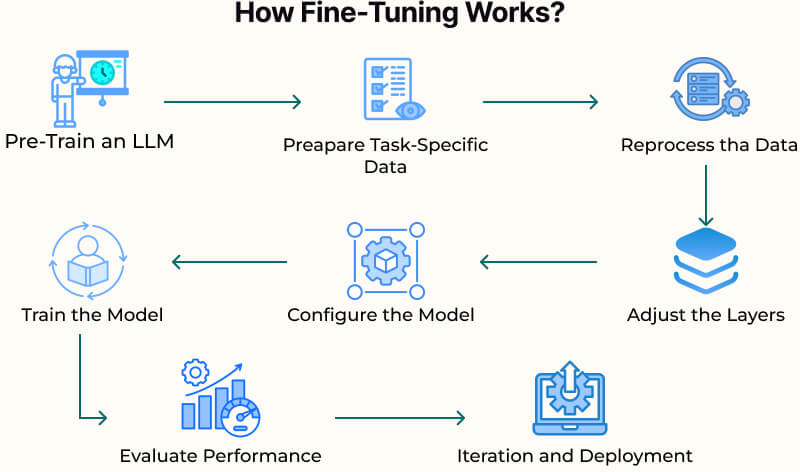
\includegraphics[height=2.3in, width=3.8in, viewport=0 0 210 118,clip]{Figures/How-Fine-Tuning-Works.jpg}
%\caption{\tiny \textrm{Pseudopotential for metallic sodium, based on the empty core model and screened by the Thomas-Fermi dielectric function.}}%(与文献\cite{EPJB33-47_2003}图1对比)
\label{How-Fine-Tuning-Works}
\end{figure}
    \begin{enumerate}
	    \item \textcolor{blue}{数据准备:}\\
		    {\fontsize{7.2pt}{6.2pt}\selectfont{收集标注特定领域数据,进行清洗和预处理,划分训练集、验证集和测试集}}
            \begin{lstlisting}[style=pythonstyle]
import pandas as pd
data = pd.read_csv('data.csv')
# 数据清洗和划分代码
            \end{lstlisting}
    \item \textcolor{red}{模型选择:}\\
	    {\fontsize{7.2pt}{6.2pt}\selectfont{根据任务需求和数据特点选择预训练模型,考虑模型大小、性能和可扩展性优先选择任务适配、参数规模合适的模型}}
    \item \textcolor{red}{微调配置:}\\
	    {\fontsize{7.2pt}{6.2pt}\selectfont{设置训练参数,如学习率、批量大小、训练轮数,选择优化器和损失函数}}
            \begin{lstlisting}[style=pythonstyle]
from torch.optim import Adam
optimizer = Adam(model.parameters(), lr = 0.001)
# 损失函数和其他配置代码
            \end{lstlisting}
    \item \textcolor{red}{模型训练:}\\
	    {\fontsize{7.2pt}{6.2pt}\selectfont{在训练集上微调模型,监控性能指标,如准确率、损失值}}
            \begin{lstlisting}[style=pythonstyle]
for epoch in range(num_epochs):
    model.train()
    # 训练步骤和指标监控代码
            \end{lstlisting}
            \begin{center}
%                \includegraphics[width=0.8\textwidth]{训练曲线}
            \end{center}
    \item \textcolor{blue}{模型评估:}\\
	    {\fontsize{7.2pt}{6.2pt}\selectfont{在验证集和测试集上评估微调后模型性能,分析评估结果}}
            \begin{lstlisting}[style=pythonstyle]
model.eval()
# 评估代码和指标计算
            \end{lstlisting}
    \end{enumerate}
    \begin{center}
%        \includegraphics[width=0.8\textwidth]{微调实现步骤图}
    \end{center}
\end{frame}

% 案例分析
\begin{frame}[allowframebreaks]
	\frametitle{案例分析~\textrm{(1)}电商领域}
商品推荐模型
            \begin{itemize}
		\setlength{\itemsep}{10pt}
                \item 案例背景:~提高推荐准确率和用户点击率
                \item 数据处理:~收集商品信息、用户行为数据,标注用户偏好,处理缺失值和异常值\\
			{\fontsize{8.2pt}{6.2pt}\selectfont{数据具有高维度、稀疏性特点}}
		\item 模型选择与微调:~选择基于\textrm{Transformer}的预训练模型\\
			{\fontsize{8.2pt}{6.2pt}\selectfont{采用全模型微调方法设置学习率\textrm{0.001},批量大小\textrm{64},训练轮数\textrm{10},训练后模型在验证集上准确率提升\textrm{10\%}}}
		\item 效果评估:~在测试集上,推荐准确率达到\textrm{80\%},用户点击率提高\textrm{20\%}\\
			{\fontsize{8.2pt}{6.2pt}\selectfont{对新用户和新商品推荐效果有待提升}}
            \end{itemize}
\end{frame}

%\begin{frame}[allowframebreaks]
%	\frametitle{案例分析~\textrm{(2)}医疗领域}
%某医院医疗大模型
%            \begin{itemize}
%		\setlength{\itemsep}{10pt}
%		    \item 案例背景:~某医院将\textrm{DeepSeek}与自研的医疗大模型深度融合,实现诊疗全流程智能化落地应用
%                \item 数据处理:~模型充分学习海量医疗指南、医学书籍等专业资料,并经千万量级临床案例指导
%		\item 模型选择与微调:~融合\textrm{DeepSeek}推理技术,兼顾系统能力和效率
%		\item 效果评估:~诊前,患者等待时间和医生问诊时间大幅缩短;~诊中,辅助医生完成诊疗记录、鉴别诊断等工作,保障诊疗质量;~诊后,帮助患者实现智能化健康管理\\
%			{\fontsize{8.2pt}{6.2pt}\selectfont{\textcolor{magenta}{如市民张女士通过该模型,仅\textrm{30}分钟就确诊为胆囊结石并制定出微创方案,诊疗效率比普通门诊提升50\%以上}}}
%            \end{itemize}
%\end{frame}
%
\begin{frame}[allowframebreaks]
	\frametitle{案例分析~\textrm{(3)}金融领域}
江苏银行\textrm{DeepSeek}模型应用
            \begin{itemize}
		\setlength{\itemsep}{10pt}
		    \item 案例背景:~江苏银行依托``智慧小苏''大语言模型服务平台,部署并微调\textrm{DeepSeek-VL2}多模态模型和轻量级的\textrm{DeepSeek-R1}推理模型
                \item 数据处理:~对海量金融数据进行深度挖掘与分析
		\item 模型选择与微调:~部署并微调\textrm{DeepSeek}系列模型,适配金融业务场景
                \item 效果评估:~为业务发展注入新动力,在复杂推理场景下实现人工智能技术应用,提升工作效率和服务质量
            \end{itemize}
\end{frame}
%
%\begin{frame}[allowframebreaks]
%	\frametitle{案例分析~\textrm{(4)}工业领域}
%奇智孔明工业大模型
%            \begin{itemize}
%		\setlength{\itemsep}{10pt}
%		    \item 案例背景:~创新奇智推出奇智孔明工业大模型\textrm{2.0}版本及多款大模型原生应用,参数量级达750亿以上,且通过中国信通院可信\textrm{AI}工业大模型评测
%		    \item 数据处理:~助力打通\textrm{AI}大模型与传统工业生产的壁垒
%                \item 模型选择与微调:~持续投入研发升级模型
%		\item 效果评估:~推出``\textrm{ChatCAD}生成式辅助工业设计''``\textrm{ChatRobot}生成式工业机器人调度''等应用前者可通过对话生成工业设计图,后者能实现对工业机器人的意念操控
%            \end{itemize}
%\end{frame}
%
\begin{frame}
	\frametitle{案例分析~\textrm{(5)}凝聚态物理与材料科学领域}
文献抽取模型
            \begin{itemize}
                \item 案例背景:~科学文献中包含大量专业术语和复杂知识\\
			{\fontsize{7.2pt}{6.2pt}\selectfont{通用大模型在处理专业文献、提取关键信息时,准确率较低,无法满足需求}}
                \item 数据处理:~研究团队收集大量凝聚态物理和材料科学领域的学术论文、研究报告等\\
			{\fontsize{7.2pt}{6.2pt}\selectfont{对文献内容进行标注,构建了包含材料结构、理化性质、实验方法、研究结论等信息的数据集;~随后对数据进行清洗,去除噪声数据和重复数据,并按照\textrm{8:1:1}的比例划分为训练集、验证集和测试集}}
		\item 模型选择与微调:~选择在自然语言处理领域表现优异的\textrm{BERT}模型作为预训练模型,借助\textrm{Hugging Face Transformers}工具,简化微调过程\\
			{\fontsize{7.2pt}{6.2pt}\selectfont{采用全模型微调方法设置学习率为\textrm{0.0001},批量大小为\textrm{32},训练轮数为\textrm{10}}}
                \item 效果评估:~微调后的模型在测试集上,大幅提高了文献分析的效率和准确性,帮助科研人员快速获取所需信息\\
			{\fontsize{7.2pt}{6.2pt}\selectfont{关键信息的抽取准确率从通用模型的\textrm{60\%}提升到了\textrm{85\%}%,召回率从50\%提升到了75%,
			}}			
            \end{itemize}
\end{frame}

\section{效果与评价}
% 大模型微调的效果评价
\begin{frame}
    \frametitle{大模型微调的效果评价}
    \begin{itemize}
	    \item \textcolor{blue}{性能提升显著:}~微调能让模型在特定任务上表现远超通用模型\\
		{\fontsize{7.2pt}{6.2pt}\selectfont{在电商推荐、医疗诊断、金融服务、工业设计等案例中,相关模型的准确率、效率等性能指标显著提高}}
	\item \textcolor{blue}{灵活性与适应性增强:}~通过微调,一个预训练大模型可适配多种不同领域和任务,降低模型开发的时间和资源成本\\
		{\fontsize{7.2pt}{6.2pt}\selectfont{同一基础模型经微调后,有可能可同时适用于多个不同场景}}
	\item \textcolor{purple}{数据需求与成本:}~尽管微调能在较小数据集上进行,但高质量的特定领域数据仍不可或缺\\
		{\fontsize{7.2pt}{6.2pt}\selectfont{全模型微调计算成本高,部分层微调或基于特征提取的微调虽能降低成本,却也可能限制模型性能的提升幅度}}
	\item \textcolor{red}{潜在风险:}~微调过程可能导致模型过拟合特定数据集,降低模型的泛化能力\\
		{\fontsize{7.2pt}{6.2pt}\selectfont{不当的微调还可能放大数据中的偏差,引发公平性和安全性等各种问题}}
    \end{itemize}
\end{frame}

%% 总结与展望
%\begin{frame}
%    \frametitle{总结与展望}
%    \begin{itemize}
%        \item **总结**:回顾大模型微调基本概念、方法、工具和实现步骤,大模型微调对定制化AI开发至关重要
%        \item **展望**:未来大模型微调将发展更高效方法、降低计算成本、拓展应用场景鼓励大家在实际工作中应用该技术
%    \end{itemize}
%    \begin{center}
%   %     \includegraphics[width=0.8\textwidth]{启发性图表}
%    \end{center}
%\end{frame}
